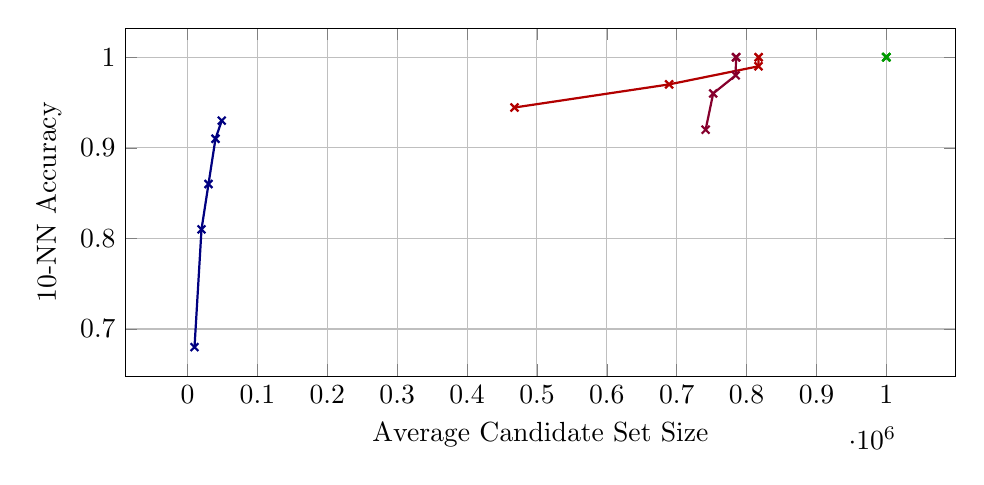
\begin{tikzpicture}
        \begin{axis}[
            width=\linewidth,
            height=6cm,
            grid=major,
            xlabel={Average Candidate Set Size},
            ylabel={10-NN Accuracy},
            mark options={solid}
        ]
        
        % Original
        \addplot[blue!50!black, thick, mark=x, mark size=2pt] coordinates {
            (10000, 0.68)
            (20000, 0.81)
            (30000, 0.86)
            (40000, 0.91)
            (49000, 0.93)
        };
        % PCA
        \addplot[red!70!black, thick, mark=x, mark size=2pt] coordinates {
            (467974, 0.9445)
            (689184, 0.97)
            (817024, 0.99)
            (817221, 1.0)
            (817221, 1.0)
        };
        % Mahalanobis
        \addplot[green!60!black, thick, mark=x, mark size=2pt] coordinates {
            (1000000, 1.0)
            (1000000, 1.0)
            (1000000, 1.0)
            (1000000, 1.0)
            (1000000, 1.0)
        };
        % Multi-model ensembling 
        \addplot[purple!70!black, thick, mark=x, mark size=2pt] coordinates {
            (741386, 0.92)
            (752203, 0.96)
            (784437, 0.98)
            (784865, 1.0)
            (785146, 1.0)
        };
        \end{axis}
\end{tikzpicture}